\documentclass[12pt,a4paper]{article}
\usepackage[utf8]{inputenc}
\usepackage{pdfpages}
\usepackage[magyar]{babel}
\usepackage{hyperref}	
\hypersetup{					
colorlinks=false,						
pdfborder={0 0 0},
}
\usepackage{fancyhdr}
\usepackage[left=2cm,right=2cm,top=3.5cm,bottom=3cm,headsep=50pt]{geometry}

\begin{document}
%=================================================
\thispagestyle{empty}
\begin{center}

\includegraphics[scale=0.3]{bme.pdf}\\
\large{Budapesti Műszaki- és Gazdaságtudományi Egyetem\\
Gépészmérnöki kar}\\[1cm]
\begin{Huge}
\textbf{Mechatronika projekt}
\end{Huge}\\[0.5cm]

\Large{BMEGEFOAMM3}\\[2cm]
\Huge{\bf{3D szkenner}}\\[2.5cm]
\bf{\Large{Tar Dániel\\[5pt]
		Bognár Máté\\
		Varga Roland}}\\[1cm]


\includegraphics[scale=0.5]{mogilogo.jpg}\\[1cm]
\large{\today}
\end{center}
%=================================================
\newpage
\tableofcontents
\newpage
\pagestyle{fancy}
\fancyhf{}
\rhead{Tar Dániel\\Bognár Máté\\Varga Roland}
\lhead{3D szkenner}
\cfoot{\thepage. oldal}
%=================================================
\section{Bevezető}
Az iparban egyre elterjedtebb a 3D szkennerek alkalmazása. Jól használhatóak gyors prototípuskészítésre és `'reverse engineering'' eljárásokhoz. Ezzel jelentős modellezési és mérési idő takarítható meg.\\[10pt]
Új eszközök tervezésénél és komplex alkatrészek méreteinek gyors meghatározására egyaránt használható. Apróbb mechanikai alkatrészek, turbinalapátok és helységek szkennelése is lehetséges adott felbontással.\\[10pt]
A gyógyászatban alkalmazzák például test vagy testrész modellezésére, mivel egyes protézisek elkészítése nagy méretpontosságot igényel, és így könnyebben formálhatóak az egyéni igények szerint.\\[10pt]
Egyetemeken régészek is használhatják leletek tanulmányozására anélkül, hogy bármilyen kártétel veszélye fennállna.\\[10pt]
\begin{figure}[h!]
\centering
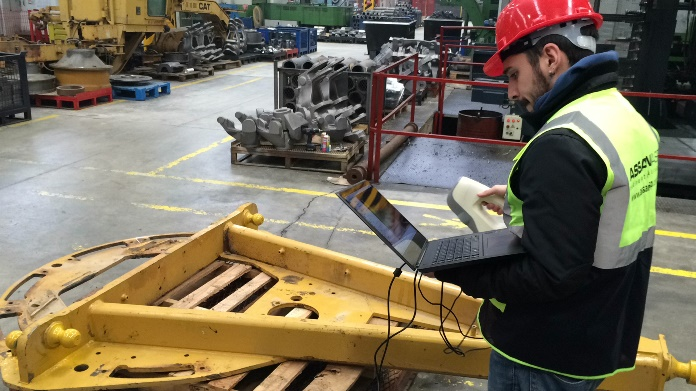
\includegraphics[height=5cm]{images/application1.jpg}
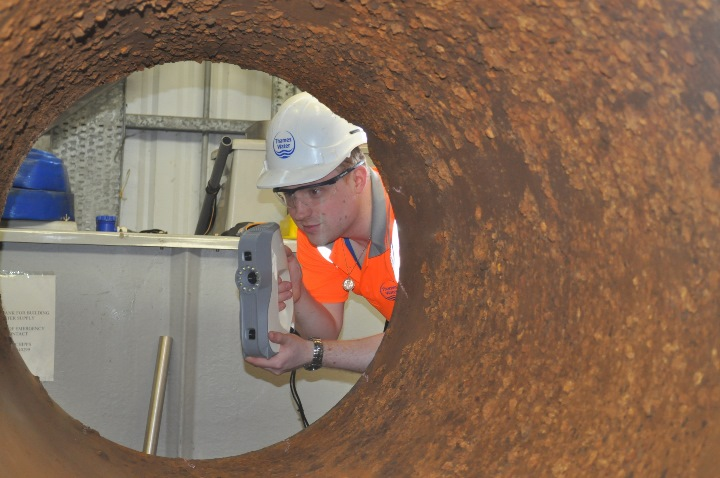
\includegraphics[height=5cm]{images/application2.jpg}
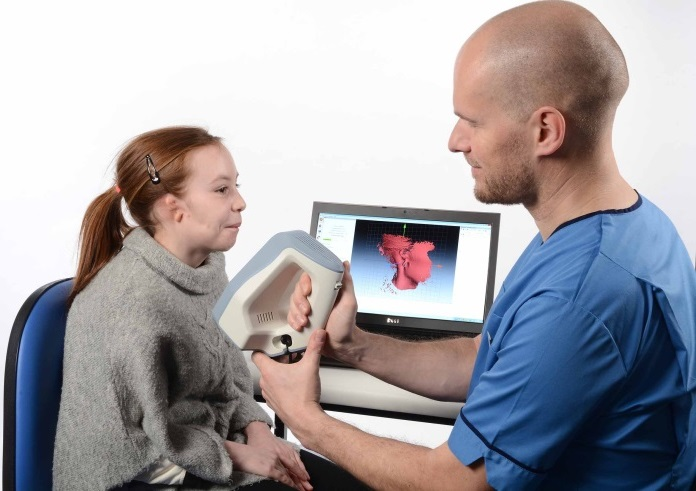
\includegraphics[height=5cm]{images/application3.jpg}
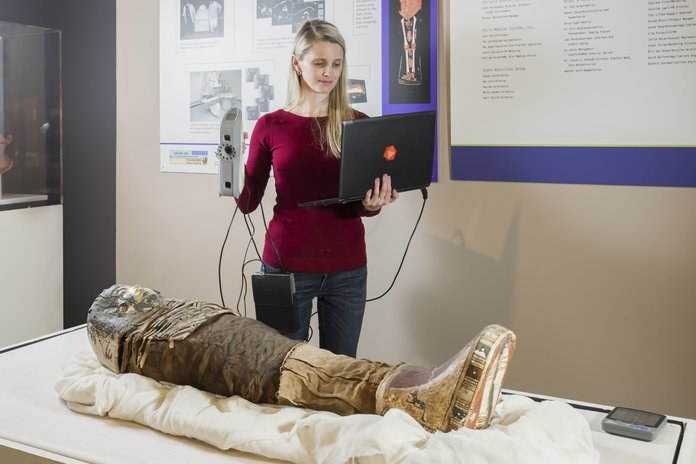
\includegraphics[height=5cm]{images/application4.jpg}
\caption{3D szkenner alkalmazása a hétköznapokban\cite{alkalmazasok}}
\end{figure}
%=================================================
\newpage
\section{Feladat leírása}
\subsection{Követelmények}
A projekt célja egy használható 3D lézerszkenner eljárás kidolgozása és megvalósítása, ami az alábbi követelményeknek megfelel:
\begin{enumerate}
	\item A konstrukció hordozhatósága: viszonylag kis befoglaló mérettel kell 			rendelkezzen és könnyen szétszerelhető-összerakható legyen.\label{hordozhatosag}
	\item A szerkezet legyen alkalmas a szerkezet együttes szabványos fényképezőállványra való rögzítésére.\label{kameraallvanyra}
	\item A megírt program átláthatóságára (felhasználóbarát) és jól dokumentáltságára kell törekedni, hogy a projektet a későbbiekben mások is tovább tudják vinni.\label{felhasznalobarat}
\end{enumerate}
\subsection{Alap koncepció}
A szkennelési módszert egy webkamera, egy vonallézer és egy forgóasztal felhasználásával dolgoztuk ki. Az eljárás lényege, hogy a tárgyra vetült lézerfény vonalról a kamerával valamekkora szögből kép készül. A képen a forgóasztal forgástengelyének meghatározhatónak kell lennie, és ez a vonallézer által meghatározott síkba kell hogy essen. A lézerpontok forgástengelytől (és azon egy tetszőleges origótól) vett távolságából a térbeli helyzetük meghatározható.
%=================================================
\section{Alapul vett szakirodalom}
Ide jönne a két nagyon hasonló projekt meghivatkozva!
%=================================================
\section{Felhasznált hardverek}
\subsection{Beszerzett eszközök}
\subsection{Saját készítésű eszközök}
\subsection{Hardverek közötti csatlakozás}
%=================================================
\section{Programkód}
Az egyes szorosan összetartozó részeket külön függvényben írtuk meg, amiket a főprogram, a scan\_object.m hív meg. A függvények csak a továbbiakban is használt változókat adják vissza, így redukáltuk a Workspace-en található vektorok számát.
\subsection{Kamera kalibráció}
\subsection{Perifériák inicializálása}
\subsection{Képek vágása}
\subsection{Transzformáció meghatározása}
\subsection{Szükséges változók deklarálása}
\subsection{Szkennelés folyamata}
\subsubsection{Lézerfény detektálása}
\subsubsection{A forgóasztal léptetése}
\subsubsection{Képek transzformációja}
\subsubsection{Pontfelhő generálása}
%=================================================
\section{Eredmények, a módszer korlátai}
%=================================================
\section{Továbbfejlesztési irányok}
%=================================================
\newpage
\begin{thebibliography}{9} 
\bibitem{feladatkiiras} 
Feladatkiírás
\href{http://mogi.bme.hu/letoltes/MECHATRONIKAI%20&%20IR%C3%81NY%C3%8DT%C3%81STECHNIKAI%20T%C3%81RGYAK/MECHATRONIKA_PROJEKT_BMEGEFOAMM3/Feladatlapok_M/}
{[link]}

\bibitem{alkalmazasok} 
3D szkennelés gyakorlati alkalmazása
\href{https://www.artec3d.com/applications}{[link]}

\end{thebibliography}

\end{document}